\PassOptionsToPackage{unicode,pdfusetitle}{hyperref}
\PassOptionsToPackage{hyphens}{url}
\PassOptionsToPackage{dvipsnames,svgnames,x11names}{xcolor}

\documentclass[10pt]{beamer}

\usetheme{moloch}
% \molochset{block=fill}
\usefonttheme{professionalfonts}
\setbeamertemplate{page number in head/foot}[appendixframenumber]

\usepackage{lmodern}
\usepackage{amssymb,amsmath,mathtools,amsthm}
\usepackage[T1]{fontenc}
\usepackage{textcomp}

\usepackage{upquote} % straight quotes in verbatim environments
\usepackage{microtype}
\UseMicrotypeSet[protrusion]{basicmath} % disable protrusion for tt fonts

\usepackage{xcolor}
\usepackage{xurl} % add URL line breaks if available
\usepackage{bookmark}
\usepackage{hyperref}

\hypersetup{%
  colorlinks = true,
  linkcolor  = mLightGreen,
  filecolor  = mLightGreen,
  citecolor  = mLightGreen,
  urlcolor   = mLightGreen
}

%% subfigures
\usepackage{caption}
\usepackage{subcaption}

% % algorithms
% \usepackage[ruled,vlined]{algorithm2e}
% \resetcounteronoverlays{algocf}

\usepackage{booktabs}

% bibliography
\usepackage[style=authoryear]{biblatex}
\addbibresource{uppsala.bib}

% title block
\titlegraphic{
\includegraphics{figures/logo.pdf}}
\title{Normalization for Class-Imbalanced Binary Features in Regularized Regression}
% \subtitle{Subtitle}
\author{Johan Larsson\\\smallskip\scriptsize \url{larssonjohan.com}, {\texttt{@jolars@fediscience.org}}}
\institute{Department of Statistics, Lund University}
\date{April 10, 2024}

% operators
\DeclareMathOperator*{\argmax}{arg\,max}
\DeclareMathOperator*{\argmin}{arg\,min}
\DeclareMathOperator{\E}{E}
\DeclareMathOperator{\var}{Var}
\DeclareMathOperator{\cov}{Cov}
\DeclareMathOperator{\tr}{tr}
\DeclareMathOperator{\diag}{diag}
\DeclareMathOperator{\range}{range}
\DeclareMathOperator{\nullspace}{null}
\DeclareMathOperator{\rank}{rank}
\DeclareMathOperator{\card}{card}
\DeclareMathOperator{\sign}{sign}
\DeclareMathOperator{\st}{S}
\DeclareMathOperator{\normal}{Normal}
\DeclareMathOperator{\fnormal}{FoldedNormal}
\DeclareMathOperator{\bernoulli}{Bernoulli}
\DeclareMathOperator{\erf}{erf}
\DeclareMathOperator{\mse}{MSE}
\DeclareMathOperator{\risk}{R}
% \DeclareMathOperator{\I}{I}
% \DeclareMathOperator{\T}{}
%
% \DeclareMathSymbol{\phi}{\mathalpha}{operators}{0}
\DeclareMathOperator{\pdf}{\phi}
\DeclareMathOperator{\cdf}{\Phi}
% commands
% \newcommand{\vec}{\vectorsym}
% \newcommand{\mat}{\matrixsym}
\renewcommand{\vec}{\boldsymbol}
\newcommand{\mat}{\boldsymbol}
\newcommand*\du{\mathop{}\!\mathrm{d}}
% \newcommand{\T}{\mathsf{T}}
\newcommand{\T}{\intercal}
\newcommand{\ones}{\boldsymbol{1}}
% \newcommand{\T}{\intercal}
% \newcommand{\T}[1]{{1}^{\mathsf{T}}}
\newcommand{\ind}[1]{\operatorname{I}_{#1}}

% environments
\theoremstyle{plain}
\newtheorem{theorem}{Theorem}[section]
\newtheorem{corollary}{Corollary}[theorem]
\newtheorem{lemma}{Lemma}[section]
\newtheorem{proposition}{Proposition}[section]

\theoremstyle{definition}
\newtheorem{definition}{Definition}[section]
\newtheorem{example}{Example}[section]

\theoremstyle{remark}
\newtheorem{remark}[theorem]{Remark}

\newcommand{\todojl}[1]{\todo[color=green!40]{#1}}



\begin{document}

\maketitle

\begin{frame}[c]
  \frametitle{Presentation}

  \begin{itemize}
    \item PhD student at Lund University (supervised by Jonas Wallin). As of September, post doc at
          Copenhagen University.
    \item Work so far: mostly computational optimization and algorithms for speeding up sparse
          regression.
  \end{itemize}
\end{frame}

\begin{frame}[c]
  \frametitle{This Talk}

  \begin{block}{Topic}
    Normalization (scaling) of binary features in regularized regression
  \end{block}

  \pause

  \begin{alertblock}{Problem}
    The elastic net (combination of lasso and ridge)
  \end{alertblock}

  \pause

  \begin{exampleblock}{Results}
    \begin{itemize}
      \item Class balance has a normalization-dependent impact on the model.
      \item In mixed datas, choice of normalization implictly biases coefficients.
    \end{itemize}
  \end{exampleblock}

  \pause

  \begin{columns}[T]
    \begin{column}{0.45\textwidth}
      \begin{block}{Notes}
        \begin{itemize}
          \item Not yet published (and partly work-in-progress)
          \item Joint work with Jonas Wallin
        \end{itemize}
      \end{block}

    \end{column}
    \begin{column}{0.45\textwidth}
      \begin{figure}
        \hfill%
        
\includegraphics[width=0.7\textwidth]{figures/jonas.jpg}
      \end{figure}
    \end{column}
  \end{columns}
\end{frame}

\begin{frame}
  \frametitle{Overview}

  \tableofcontents
\end{frame}

\section{Preliminaries}

\begin{frame}
  \frametitle{General Setup}

  \begin{itemize}
    \item Data consists of a \alert{fixed} matrix of features \(\mat{X} \in \mathbb{R}^{n \times p}\)
          and a response vector \(\vec{y} \in \mathbb{R}^n\).
    \item \(\vec{y}\) comes from a linear model, that is,
          \[
            y_i = \beta_0^* + \vec x_i^\T \vec\beta^* + \varepsilon_i \quad\text{for} \quad i \in 1,\dots,n,
          \]
          where \(\vec{\beta}^*\) is the vector of \emph{true} coefficients.
    \item \(\varepsilon_i\) is the measurement noise, generated from some random variable
  \end{itemize}
\end{frame}

\begin{frame}[c]
  \frametitle{The Elastic Net}

  Linear regression plus a combination of the \(\ell_1\) and \(\ell_2\) penalties:
  \begin{equation*}
    (\hat{\beta}_0, \hat{\vec{\beta}}) = \argmin_{\beta_0 \in \mathbb{R},\beta \in \mathbb{R}^p} \left( \frac{1}{2} \lVert \vec y - \beta_0 - \mat{X}\vec{\beta} \rVert^2_2  + \lambda_1 \lVert \vec\beta \rVert_1 + \frac{\lambda_2}{2}\lVert \vec \beta \rVert_2^2\right).
  \end{equation*}

  \pause

  \begin{figure}
    \centering
    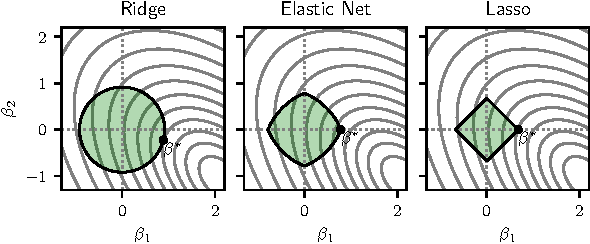
\includegraphics[]{figures/elasticnet-balls.pdf}
    \caption{%
      The elastic net penalty is a combination of the lasso and ridge penalties. Here shown as a constrained problem.
    }
  \end{figure}

  % TODO: Insert figure of elastic net, ridge, lasso here. Possibly just the constraint regions?
\end{frame}

\begin{frame}[c]
  \frametitle{The Elastic Net Path}

  \begin{columns}
    \begin{column}{0.45\textwidth}
      \begin{itemize}[<+->]
        \item Usually don't know optimal \(\lambda_1\) and \(\lambda_2\) in advance.
        \item Instead we typically hyper-optimize (e.g. cross-validate) over a grid.
        \item Common parametrization:
              \begin{align*}
                \lambda_1 & = \alpha\lambda,     \\
                \lambda_2 & = (1- \alpha)\lambda
              \end{align*}
              with \(\alpha \in [0, 1]\).
        \item For each \(\alpha\), solve the elastic net over a sequence of \(\lambda\): the
              \textbf{elastic net path}.
      \end{itemize}
    \end{column}
    \begin{column}{0.45\textwidth}
      \only<4->{%
        \begin{figure}[htpb]
          \centering
          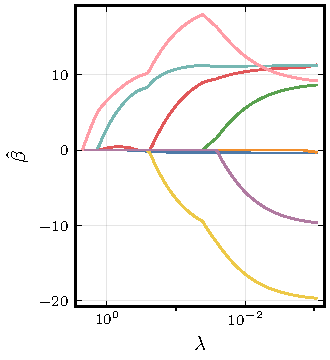
\includegraphics[]{figures/elasticnet_path.pdf}
          \caption{%
            The elastic net path
          }
        \end{figure}
      }
    \end{column}
  \end{columns}

\end{frame}

\begin{frame}[c]
  \frametitle{Background on the Elastic Net}

  \begin{itemize}
    \item<1-> Proposed by \citet{zou2005}.
    \item<2-> Lasso (\(\ell_1\)) part:
          \begin{itemize}
            \item Enables sparsity (interpretability, parsimony, feature selection)
            \item Efficient when \(p \gg n\) (due to screening rules~\citep{elghaoui2010,tibshirani2012})
          \end{itemize}
    \item<3-> Ridge (\(\ell_2\)) part
          \begin{itemize}
            \item Mitigates lasso issue in correlated data
            \item Better predictive performance when true signal is non-sparse
          \end{itemize}
    \item<4-> Very efficient solvers for the full path (coordinate descent)
  \end{itemize}
\end{frame}

\begin{frame}[c]
  \frametitle{Sensitivity to Scale}

  Since both the lasso and ridge penalize the \emph{norm} of the coefficients, they are
  sensitive to the scale of the features.

  \pause

  \begin{exampleblock}{Example}
    Assume
    \[
      \mat{X} \sim \operatorname{Normal}\left(\begin{bmatrix}0 \\ 0\end{bmatrix}, \begin{bmatrix} 2 & 0 \\ 0 & 1\end{bmatrix}\right), \qquad \vec{\beta}^* = \begin{bmatrix} \frac{1}{2} \\ 1 \end{bmatrix}.
    \]

    \medskip\pause

    \begin{table}
      \begin{tabular}{lcc}
        \toprule
        Model & \(\hat{\vec{\beta}}\)                                  & \(\hat{\vec{\beta}}_\text{std}\)                      \\
        \midrule
        OLS   & \(\begin{bmatrix} 0.50 & 1.00\end{bmatrix}^\intercal\) & \(\begin{bmatrix}1.00 & 1.00\end{bmatrix}^\intercal\) \\
        Lasso & \(\begin{bmatrix} 0.38 & 0.50\end{bmatrix}^\intercal\) & \(\begin{bmatrix}0.74 & 0.50\end{bmatrix}^\intercal\) \\
        Ridge & \(\begin{bmatrix} 0.37 & 0.41\end{bmatrix}^\intercal\) & \(\begin{bmatrix}0.74 & 0.41\end{bmatrix}^\intercal\) \\
        \bottomrule
      \end{tabular}
    \end{table}
  \end{exampleblock}

  \pause

  \alert{Large} scale means \alert{less} penalization because the size of \(\beta_j\) can be smaller for an equivalent effect (on \(\vec{y}\)).

\end{frame}

\begin{frame}[c]
  \frametitle{Normalization}

  \begin{itemize}[<+->]
    \item The solution to the scale sensitivity is to normalized the features (before fitting).
    \item Let \(\tilde{\mat X}\) be the normalized feature matrix, with elements
          \[
            \tilde{x}_{ij} = \frac{x_{ij} - c_{j}}{s_j},
          \]
          where \(x_{ij}\) is an element of the (unnormalized) feature matrix and \(c_j\) and \(s_j\)
          are the \emph{centering} and \emph{scaling} factors respectively.
    \item Usage of key terms ambiguous in literature.
    \item After fitting, we transform the coefficients back to their original scale via
          \[
            \hat\beta_j = \frac{\hat\beta^{(n)}_j}{s_j} \quad\text{for}\quad j = 1,2,\dots,p.
          \]

  \end{itemize}

  % \bigskip\pause
  % \begin{block}{Ambiguous Nomenclature}
  %   \begin{itemize}
  %     \item Some refer to this as \emph{standardization} (which we dedicate for the mean--standard deviation combo).
  %     \item Some take normalization to mean \alert{sample-wise} normalization.
  %     \item Some take normalization to mean scaling with a \alert{norm}.
  %     \item Some refer to this (centering and scaling) as \alert{scaling}.
  %   \end{itemize}
  % \end{block}
\end{frame}

\begin{frame}[c]
  \begin{table}[hbt]
    \centering
    \caption{Common ways to normalize \(\mat{X}\)}
    \begin{tabular}{lll}
      \toprule
      Normalization    & Centering (\(c_{j}\))                          & Scaling (\(s_j\))                                         \\
      \midrule
      Standardization  & \(\bar{x}_j = \frac{1}{n}\sum_{i=1}^n x_{ij}\) & \(\sqrt{\frac{1}{n}\sum_{i=1}^n (x_{ij} - \bar{x}_j)^2}\) \\
      \addlinespace
      Min--Max         & \(\min_i(x_{ij})\)                             & \(\max_i(x_{ij}) - \min_i(x_{ij})\)                       \\
      \addlinespace
      Unit Vector (L2) & 0                                              & \(\sqrt{\sum_{i=1}^n x_{ij}^2}\)                          \\
      \addlinespace
      Max--Abs         & 0                                              & \(\max_i(|x_{ij}|)\)                                      \\
      \addlinespace
      Adaptive Lasso   & 0                                              & \(\beta_j^\text{OLS}\)                                    \\
      \bottomrule
    \end{tabular}
  \end{table}
\end{frame}

\section{Motivation}

\begin{frame}[c]
  \frametitle{The Type of Normalization Matters}

  \begin{figure}[htpb]
    \centering
    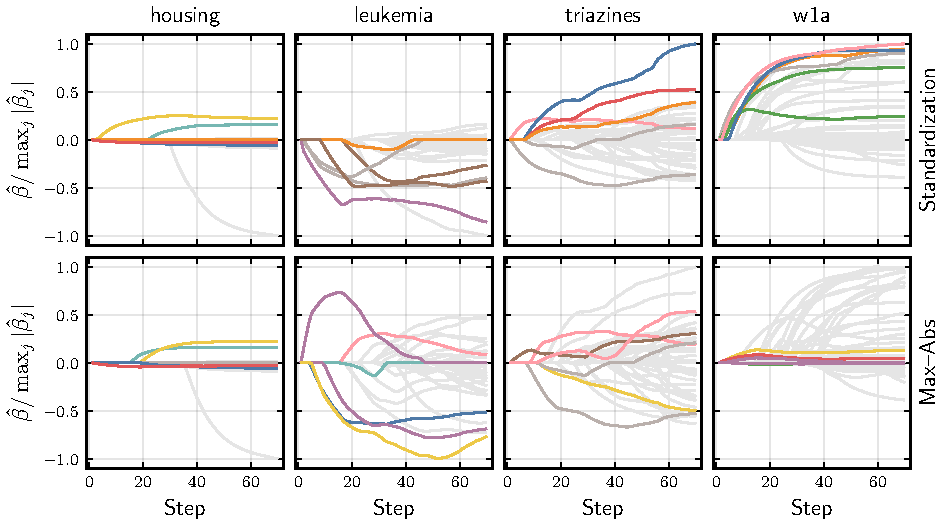
\includegraphics[width=\textwidth]{figures/realdata_paths.pdf}
    \caption{%
      Lasso paths under two different types of normalization (standardization and max--abs normalization). The union of the first ten features selected in any of the schemes are colored.
    }
  \end{figure}

\end{frame}

\begin{frame}[c]
  \frametitle{Motivation}

  \begin{itemize}[<+->]
    \item So normalization matters and you might expect that there should be lot of literature on the
          topic.
    \item But the short summary of the literature on the topic is that there is no literature on the
          topic.
    \item Everyone agrees that you need to normalize (for most data), but how to do so is not
          discussed and often motivated by being ``standard''.
    \item Documentation for popular machine learning packages advocate different normalization
          strategies when data is sparse.
    \item Consensus for approximately normal features but little discussion on binary features and
          choice seems domain-specific. (Statisticians standardize, machine learning people scale to
          $[0, 1]$ or $[-1, 1]$.)
  \end{itemize}
\end{frame}

\begin{frame}
  \frametitle{Aims}

  We focus on the following aspects of normalization in the context of the elastic net:
  \begin{itemize}
    \item Binary features, particularly with respect to the \alert{class balance} thereof
    \item A mix of binary and normally distributed features
    \item Interactions
  \end{itemize}

  % \begin{block}{Findings}
  %   \begin{itemize}
  %     \item Class-balance in binary features has a fundamental role in the expected value of the coefficients, especially for the lasso.
  %     \item Normalization can mitigate this effect, but at the price of increased variance.
  %     \item I.e. there is a bias--variance trade off in the choice of normalization.
  %     \item For mixed data, the choice of normalization imposes an implicit
  %   \end{itemize}
  % \end{block}

\end{frame}

\section{Results}

\begin{frame}[c]
  \frametitle{Orthogonal Features}

  There is not an explicit solution to the elastic net problem in general (unless \(\lambda_1
  = 0\)).

  \bigskip\pause

  \begin{columns}
    \begin{column}{0.45\textwidth}
      But if we assume that the features are orthogonal, that is
      \[
        \tilde{\mat{X}}^\intercal \tilde{\mat{X}} = \diag(\tilde{\vec{x}}_1^\intercal \tilde{\vec{x}}_1, \dots, \tilde{\vec{x}}_p^\intercal \tilde{\vec{x}}_p),
      \]
      then there is an explicit solution to the elastic net problem\footnote[frame]{We have also
        assumed that the features are mean-centered here.}:
      \begin{equation*}
        \hat\beta_j = \frac{\st_{\lambda_1}\left(\tilde{\vec{x}}_j^\T \vec{y}\right)}{s_j\left(\tilde{\vec{x}}_j^\T \tilde{\vec{x}}_j + \lambda_2\right)},
      \end{equation*}
      where
      \[
        \st_\lambda(z) = \sign(z) \max(|z| - \lambda, 0).
      \]\pause
    \end{column}
    \begin{column}{0.45\textwidth}
      \begin{figure}[htpb]
        \centering
        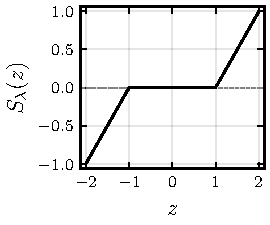
\includegraphics[]{figures/soft-thresholding.pdf}
        \caption{%
          Soft thresholding
        }
      \end{figure}
    \end{column}
  \end{columns}

\end{frame}

\begin{frame}[c]
  \frametitle{Bias and Variance of the Elastic Net Estimator}

  The goal is computing the expected value of the elastic net estimator,
  \[
    \E \hat\beta_j = \frac{\E \st_{\lambda_1}\left(\tilde{\vec{x}}_j^\T \vec{y}\right)}{s_j\left(\tilde{\vec{x}}_j^\T \tilde{\vec{x}}_j + \lambda_2\right)},
  \]
  since we treat \(\mat{X}\) as fixed.

  \bigskip\pause

  Letting \(Z = \tilde{\vec{x}}^\intercal \vec{y}\) and assuming that \(\varepsilon_i\) is
  i.i.d. with mean zero and finite variance \(\sigma_\varepsilon^2\), we have
  \begin{align*}
    \E Z   & = \mu = \E \left( \tilde{\vec{x}}_j^\T (\vec{x}_j\beta_j + \vec{\varepsilon}) \right)  = \tilde{\vec{x}}_j^\T\vec{x}_j \beta_j,  \\
    \var Z & = \sigma^2 = \var\left(\tilde{\vec{x}}_j ^\T \vec{\varepsilon}\right) = \sigma_\varepsilon^2 \lVert \tilde{\vec{x}}_j\rVert_2^2.
  \end{align*}

  \bigskip

  Next, will will turn to \(\E \st_{\lambda_1}(Z)\).
\end{frame}

\begin{frame}[c]
  \frametitle{Bias of Soft-Thresholding}

  \begin{columns}
    \begin{column}{0.45\textwidth}
      The expected value of the soft-thresholding estimator is
      \begin{align*}
         & \E \st_\lambda(Z)                                                                                               \\
         & = \int_{-\infty}^\infty \st_\lambda(z) f_Z(z) \du z                                                   \nonumber \\
        % & = \int_{-\infty}^\infty \ind{|z| > \lambda} (z -\sign(z)\lambda) f_Z(z) \du z                         \nonumber \\
         & = \int_{-\infty}^{-\lambda}(z + \lambda)f_Z(z) \du z                                                            \\
         & \phantom{=} + \int_{\lambda}^\infty (z - \lambda)f_Z(z) \du z.
      \end{align*}
      And so the bias of \(\hat\beta_j\)  is
      \begin{equation*}
        \E \hat\beta_j - \beta_j^* = \frac{1}{d_j}\E \st_\lambda(Z) - \beta^*_j.
      \end{equation*}
    \end{column}
    \begin{column}{0.45\textwidth}
      \begin{figure}[htpb]
        \centering
        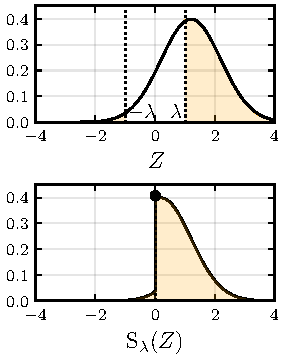
\includegraphics[]{figures/z_normal.pdf}
        \caption{%
          Distributions of \(Z\) and the its value after soft-thresholding.
        }
      \end{figure}
    \end{column}
  \end{columns}

\end{frame}

\begin{frame}[c]
  \frametitle{Variance of Soft-Thresholding}

  The variance of the soft-thresholding estimator is
  \begin{equation*}
    \var {S_\lambda(Z)} = \int_{-\infty}^{-\lambda}(z + \lambda)^2f_Z(z) \du z + \int_{\lambda}^\infty (z - \lambda)^2 f_Z(z) \du z - \left(\E \st_\lambda(Z)\right)^2
  \end{equation*}
  and consequently the variance of the elastic net estimator is therefore
  \begin{equation*}
    \var \hat\beta_j = \frac{1}{d_j^2} \var \st_\lambda(Z).
  \end{equation*}

\end{frame}

\begin{frame}[c]
  \frametitle{Normally Distributed Noise}

  We now assume that \(\varepsilon_i \sim \normal{(0, \sigma_\varepsilon^2)}\), which means
  that
  \[
    Z \sim \normal\left(\tilde{\vec{x}}_j^\T\vec{x}_j \beta_j, \sigma_\varepsilon^2 \lVert \tilde{\vec{x}}_j\rVert_2^2 \right).
  \]

  Let \(\theta = -\mu -\lambda_1 \) and \(\gamma = \mu - \lambda_1\). Then the expected value
  of soft-thresholding of \(Z\) is
  \begin{align*}
    \E \st_{\lambda_1}(Z) & = \int_{-\infty}^\frac{\theta}{\sigma} (\sigma u - \theta) \pdf(u) \du u + \int_{-\frac{\gamma}{\sigma}}^\infty (\sigma u + \gamma) \pdf(u) \du u                                               \nonumber \\
                          & = -\theta \cdf\left(\frac{\theta}{\sigma}\right) - \sigma \pdf\left(\frac{\theta}{\sigma}\right) + \gamma \cdf\left(\frac{\gamma}{\sigma}\right) + \sigma \pdf\left(\frac{\gamma}{\sigma}\right)
  \end{align*}
  where \(\pdf(u)\) and \(\cdf(u)\) are the pdf and cdf of the standard normal distribution, respectively.

  \bigskip\pause

  Similar, but more complicated, expression can be derived for \(\var \st_{\lambda_1}(Z)\).

\end{frame}

\begin{frame}[c]
  \frametitle{Binary Features}

  Let's say we have a binary feature \(\vec{x}_j\), such that \(x_{ij} \in \{0, 1\}\). Let
  \(q \in [0, 1]\) be the class balance of this feature, that is: \(q = \bar{\vec{x}}_j\).

  \bigskip

  In this case, we observe that
  \[
    \begin{aligned}
      \tilde{\vec{x}}_j^\T \tilde{\vec{x}}_j & = \frac{1}{s_j^2}(\vec{x}_j - \ones c_j)^\T (\vec{x}_j - \ones c_j) = \frac{1}{s^2_j}(nq - 2nq^2 + nq^2) = \frac{n(q-q^2)}{s^2_j}, \\
      \tilde{\vec{x}}_j^\T \vec{x}_j         & = \frac{1}{s_j}(\vec{x}_j^\T \vec{x}_j - \vec{x}_j^\T \ones c_j) = \frac{n(q - q^2)}{s_j}.
    \end{aligned}
  \]
  \pause%
  And consequently
  \[
    \mu = \frac{\beta^*_j n(q - q^2)}{s_j}, \qquad \sigma^2 = \frac{\sigma_\varepsilon^2n(q - q^2)}{s^2_j}, \qquad d_j = \frac{n(q -q^2)}{s_j}  + \lambda_2 s_j.
  \]
\end{frame}

\begin{frame}[c]
  \frametitle{Noiseless Case}

  In the noiseless case, we have
  \[
    \hat{\beta}_j = \frac{\st_{\lambda_1}(\tilde{\vec{x}}^\intercal \vec{y})}{s_j\left(\tilde{\vec{x}}_j^\intercal \tilde{\vec{x}}_j + \lambda_2\right)}
    =
    \frac{\st_{\lambda_1}\left(\frac{\beta_j^* n (q - q^2)}{s_j}\right)}{s_j\left(\frac{n(q - q^2)}{s_j^2} + \lambda_2\right)}.
  \]
  \pause
  \begin{itemize}[<+->]
    \item Means that the elastic net estimator depends on class balance (\(q\)).
    \item To remove the effect of \(q\), an intuitive setting would be \(s_j = q - q^2\) (the
          variance of \(\vec{x}_j\)) in the case of the lasso and \(s_j = \sqrt{q-q^2}\) (the
          standard deviation of \(\vec{x}_j\)) in the case of the ridge.
    \item Suggests the parametrization
          \[
            s_j = (q - q^2)^\delta, \qquad \delta \geq 0.
          \]
    \item Indicates there might be no (simple) \(s_j\) that will work for the elastic net.
  \end{itemize}
  % \pause
  % \begin{block}{Scaling Parametrization}
  %   We are going to use the scaling parametrization
  %   \[
  %     s_j = (q - q^2)^\delta, \qquad \delta \geq 0.
  %   \]
  % \end{block}
\end{frame}

\begin{frame}[c]
  \frametitle{Probability of Selection}

  Since \(\mat{X}\) is fixed and \(\vec{\varepsilon}\) is normal, it is straightforward to
  compute the probability of selection:
  \[
    \Pr(\hat{\beta}_j \neq 0) = \cdf\left(\frac{\mu - \lambda_1}{\sigma}\right) + \cdf\left(\frac{- \mu -\lambda_1}{\sigma}\right).
  \]

  \begin{figure}[htpb]
    \centering
    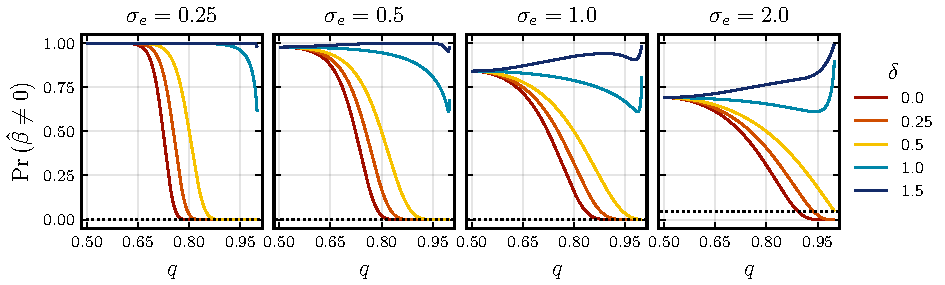
\includegraphics[width=\textwidth]{figures/selection_probability.pdf}
    \caption{%
      Probability that the elastic net selects a feature across different noise levels \((\sigma_\varepsilon)\), types of normalization (\(\delta\)), and class balance (\(q\)).
      The dashed line is asymptotic behavior for \(\delta = 1/2\).
    }
  \end{figure}
\end{frame}

\begin{frame}[c]
  \frametitle{Asymptotic Results for Bias and Variance}

  \begin{theorem}
    If \(\vec{x}_j\) is a binary feature with class balance \(q \in (0, 1)\) and \(\lambda_1,\lambda_2 \in (0,\infty)\), \(\sigma_\varepsilon > 0\), and \(s_j = (q - q^2)^{\delta}\), \(\delta \geq 0\), then
    \[
      \lim_{q \rightarrow 1^-} \E \hat{\beta}_j =
      \begin{cases}
        0                                                                                                  & \text{if } 0 \leq \delta < \frac{1}{2}, \\
        \frac{2n \beta_j^*}{n + \lambda_2} \cdf\left(-\frac{\lambda_1}{\sigma_\varepsilon \sqrt{n}}\right) & \text{if } \delta = \frac{1}{2},        \\
        \beta^*_j                                                                                          & \text{if } \delta \geq \frac{1}{2}.
      \end{cases}
    \]
    \pause and
    \[
      \lim_{q \rightarrow 1^-} \var \hat{\beta}_j =
      \begin{cases}
        0      & \text{if } 0 \leq \delta < \frac{1}{2}, \\
        \infty & \text{if } \delta \geq \frac{1}{2}.
      \end{cases}
    \]
  \end{theorem}

\end{frame}

\begin{frame}[c]
  \frametitle{A Bias--Variance Tradeoff}

  \begin{figure}
    \centering
    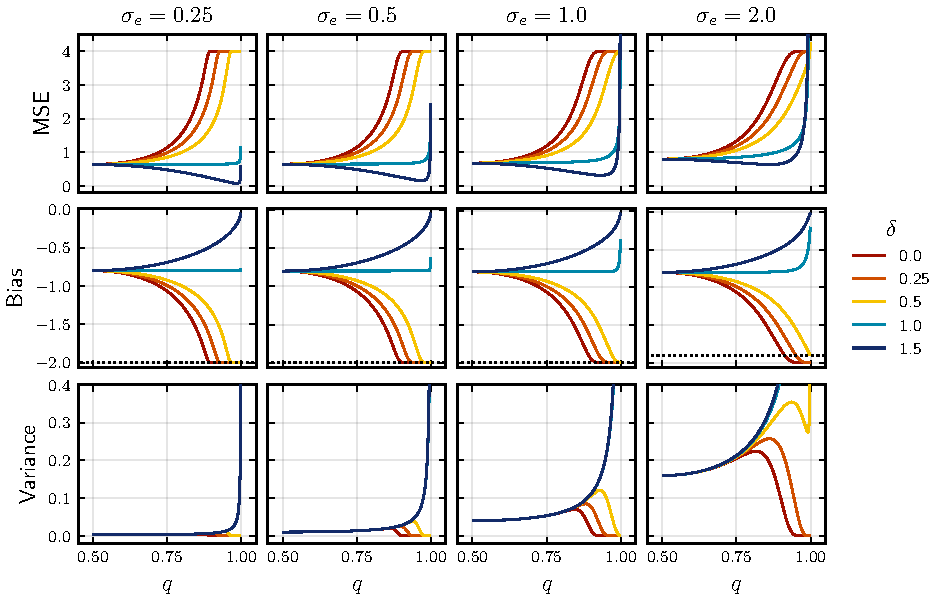
\includegraphics[width=0.94\textwidth]{figures/bias-var-onedim.pdf}
    \caption{%
      Bias, variance, and mean-squared error for a one-dimensional lasso problem. Theoretical result for orthogonal features. Dotted line is asymptotic result or \(\delta = 1/2\).
    }
  \end{figure}

\end{frame}

\begin{frame}[c]
  \frametitle{Multiple Features: Power, FDR, and NMSE}

  Lasso example with 10 true signals and varying \(q\) and \(p\).

  \begin{figure}[htpb]
    \centering
    \subcaptionbox{%
      Power in the sense of detecting all the true signals. Constant \(p\).
    }{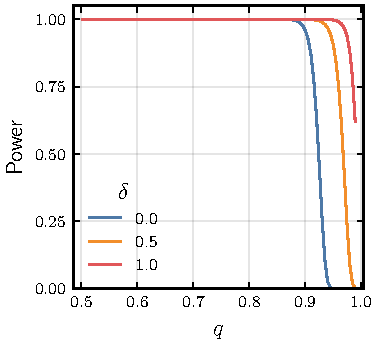
\includegraphics[width=0.35\textwidth]{figures/power.pdf}}\hfill\pause%
    \subcaptionbox{%
      False discovery rate (FDR) and normalized mean-squared error (NMSE).
    }{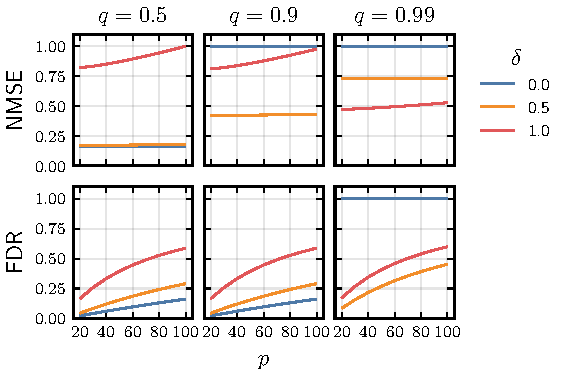
\includegraphics[width=0.55\textwidth]{figures/fdr_mse.pdf}}
    \caption{%
      Mean squared error (MSE), false discovery rate (FDR), and power.
    }
  \end{figure}
\end{frame}

\begin{frame}[c]
  \frametitle{Mixed Data}

  \textbf{So far:} \alert{all} binary features. What about mixing binary and continuous (normal) features?

  \medskip

  How to put binary features and normal features on the ``same'' scale?

  \medskip\pause

  \begin{block}{Our Definition of Comparability}
    The effects of a binary feature and a normally distributed feature are \alert{comparable} if a flip in the binary feature has the same effect as a two-standard deviation change in the normal feature~\citep{gelman2008}.
  \end{block}

  \pause

  \begin{exampleblock}{Examples}
    Assume entries in \(\vec{x}_1\) are binary and \(\vec{x}_2\) come from a random variable \(X_2\). The effects are comparable in the following cases:
    \begin{itemize}
      \item \(X_2 \sim \normal(\mu, 1/2)\), \(\beta_1^* = 1\), and \(\beta_2^* = 1\).
      \item \(X_2 \sim \normal(\mu, 2)\), \(\beta_1^* = 1\), and \(\beta_2^* = 0.25\).
    \end{itemize}
  \end{exampleblock}

  \pause

  \begin{block}{Additional Scaling}
    To account for this, we need to invoke additional scaling.

  \end{block}
\end{frame}

\begin{frame}[c]
  \frametitle{Choice of Scaling in Mixed Data}

  For the two-standard deviation notion of comparability to hold, we need to modify our
  scaling factor \(s_j\).

  \bigskip\pause

  As before, we assume that \(\vec{x}_1\) is binary and \(X_2 \sim \normal(\mu, 1/2)\),
  \(\beta_1^* = \beta_2^* = 1\) so that they have \emph{comparable} effects. Also assume we
  standardize \(\vec{x}_2\).

  \medskip

  We want \(\hat{\beta}_1 = \hat{\beta}_2\). That is,
  \[
    \underbrace{\frac{\st_{\lambda_1}\left(\frac{n (q - q^2)}{s_j}\right)}{s_1\left(\frac{n(q - q^2)}{s_1^2} + \lambda_2\right)}}_{\hat{\beta}_1}  = \underbrace{\frac{\st_{\lambda_1}\left(\frac{n}{2}\right)}{\frac{1}{2}\left(n + \lambda_2\right)}}_{\hat{\beta}_2}.
  \]

  \medskip\pause

  The choice \(s_1 = (2 (q - q^2))^\delta\) works when classes are balanced (\(q = 0.5\)).
  But no clear chocie for the elastic net case.
\end{frame}

\section{Experiments}

\begin{frame}[c]
  \frametitle{Binary Features}
  \framesubtitle{Decreasing \(q\)}

  \begin{figure}[htpb]
    \centering
    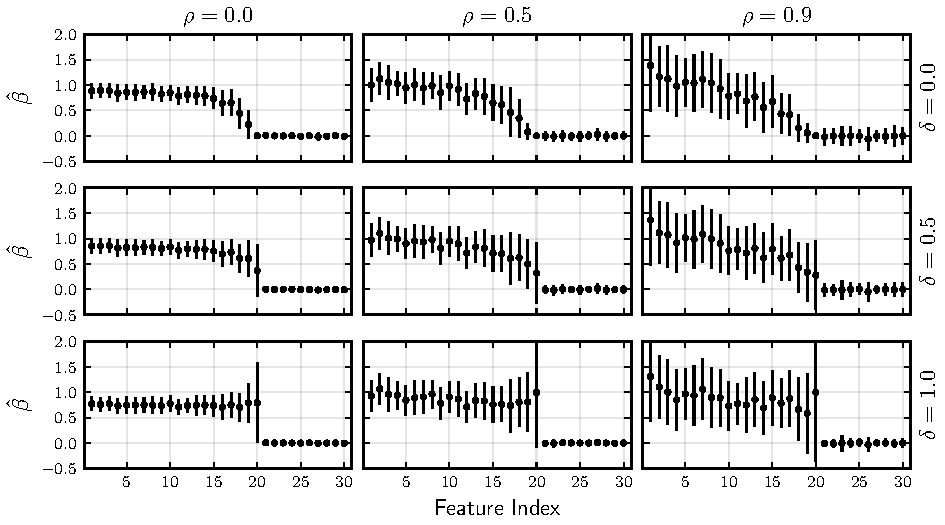
\includegraphics[width=\textwidth]{figures/binary_decreasing.pdf}
    \caption{%
      Lasso estimates for first 30 coefficients. First 20 features are true signals with a geometrically decreasing class balance from 0.5 to 0.99.
    }
  \end{figure}
\end{frame}

\begin{frame}[c]
  \frametitle{Binary Features}
  \framesubtitle{Signal-to-Noise Ratio}

  \begin{figure}[htpb]
    \centering
    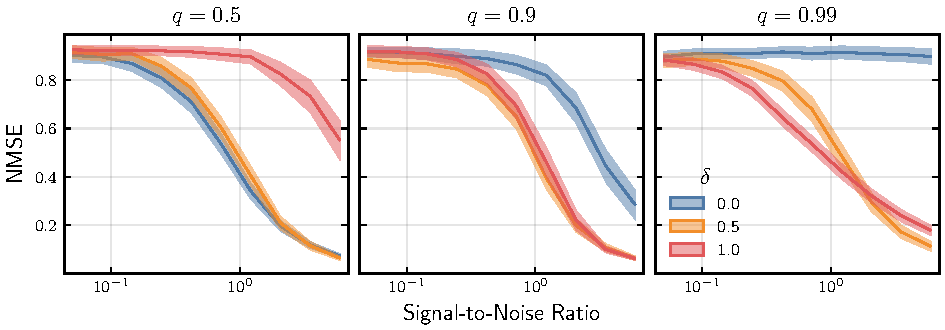
\includegraphics[width=\textwidth]{figures/binary_data_sim.pdf}
    \caption{%
      Normalized mean-squared test set error (NMSE).
    }
  \end{figure}
\end{frame}

\begin{frame}[c]
  \frametitle{Mixed Data}

  \begin{figure}[htpb]
    \centering
    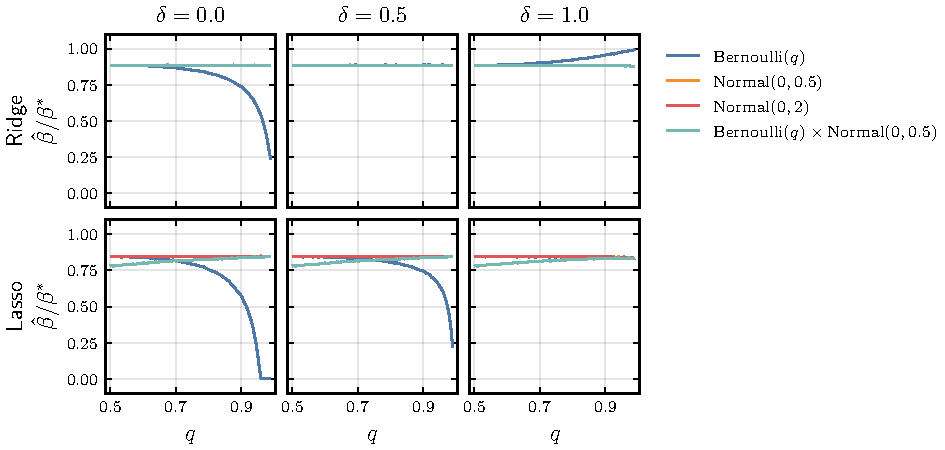
\includegraphics[width=\textwidth]{figures/mixed_data.pdf}
    \caption{%
      Comparison between lasso and ridge estimators for features generated to resemble features from various distributions.}
  \end{figure}
\end{frame}

\begin{frame}[c]
  \frametitle{Hyperparameter Optimization}

  \textbf{Idea:} The choice of \(\delta\) affects the model, so let's optimize over it.

  \begin{figure}[htpb]
    \centering
    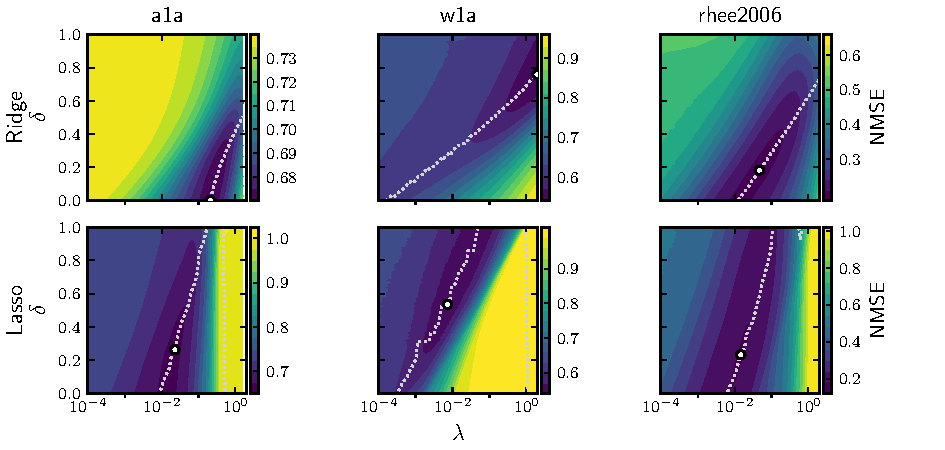
\includegraphics[width=\textwidth]{figures/hyperopt_surfaces.pdf}
    \caption{%
      Contour plots of hold-out (validation set) error across a grid of \(\delta\) and \(\lambda\) values for the
      lasso and ridge.
    }
  \end{figure}

\end{frame}

\begin{frame}[c]
  \frametitle{Hyperparameter Optimization}
  \framesubtitle{Support and NMSE}

  \begin{figure}[htpb]
    \centering
    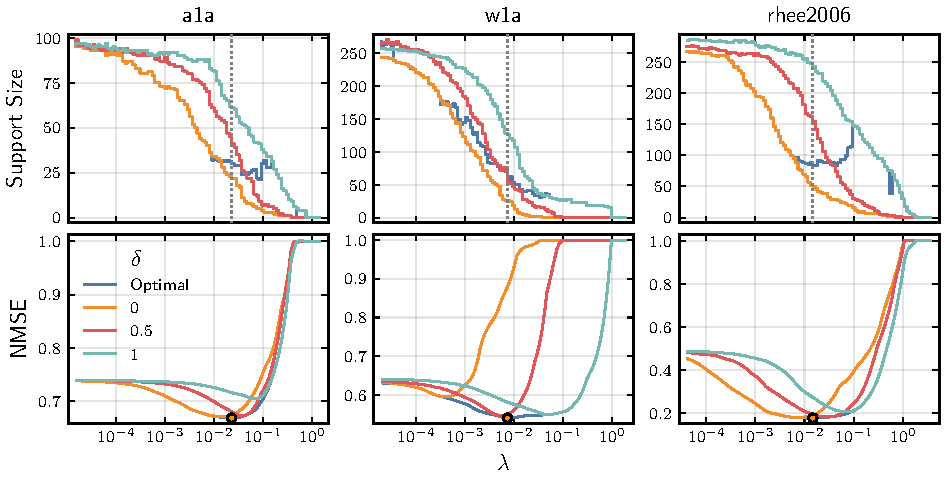
\includegraphics[width=\textwidth]{figures/hyperopt_paths.pdf}
    \caption{%
      Support and NMSE of the lasso for different values of \(\delta\) and \(\lambda\).
    }
  \end{figure}
\end{frame}

\begin{frame}[c]
  \frametitle{Interaction Effects}

  \begin{figure}[htpb]
    \centering
    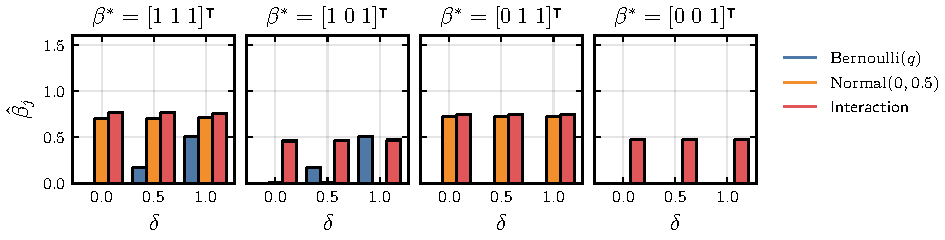
\includegraphics[width=\textwidth]{figures/interactions.pdf}
    \caption{%
      The effect of different normalization strategies for mixed data with interactions.
    }
  \end{figure}

  \pause

  \begin{exampleblock}{Open Questions}
    \begin{itemize}
      \item How to deal with features with different locations?
      \item Should the interaction features be normalized conditionally?
    \end{itemize}
  \end{exampleblock}
\end{frame}

\begin{frame}[c]
  \frametitle{Conclusions}
  \begin{exampleblock}{Conclusions}
    \begin{itemize}
      \item Class balance plays a crucial role for binary features.
      \item Effect depends on penalty
      \item Normalization mediates this effect at the cost of increased variance.
      \item Need to consider the notion of comparability between normal and binary features in mixed
            data.
    \end{itemize}
  \end{exampleblock}

  \pause

  \begin{alertblock}{Future Research}
    \begin{itemize}
      \item Random \(\mat{X}\)
      \item Theory for \(\mat{X}\) with correlation structure
      \item Non-Gaussian continuous features
      \item Other loss functions (GLMs, hinge loss, neural networks)
      \item Other penalties (group lasso, SCAD, MCP, SLOPE)
    \end{itemize}
  \end{alertblock}
\end{frame}

\begin{frame}[standout]
  Thank you!
\end{frame}

\appendix

\begin{frame}[allowframebreaks]{References}
  \printbibliography[heading=none]
\end{frame}

\section{Extras}

\begin{frame}[c]
  \frametitle{Max--Abs Scaling of Continuous Features}

  \begin{columns}
    \begin{column}{0.45\textwidth}

      \begin{itemize}
        \item Min--max normalization is sometimes used in continuous data
        \item Very sensitive to outliers
        \item But also depend on sample size!
        \item In other words, results in model validation with varying sample sizes can yield very
              strange results.
      \end{itemize}

      % \begin{theorem}
      %   Let \(X_1, X_2, \dots, X_n\) be a sample of normally distributed random variables, each with mean \(\mu\) and standard deviation \(\sigma\). Then
      %   \[
      %     \lim_{n \rightarrow \infty}\Pr\left(\max_{i \in [n]} |X_i| \leq x\right) = G(x),
      %   \]
      %   where \(G\) is the cumulative distribution function of a Gumbel distribution with
      %   parameters
      %   \[
      %     b_n = F_Y^{-1}(1 - 1/n)\quad \text{and} \quad a_n = \frac{1}{n f_Y(\mu_n)},
      %   \]
      %   where \(f_Y\) and \(F_Y^{-1}\) are the probability distribution function and quantile function, respectively, of a folded normal distribution with mean \(\mu\) and standard deviation \(\sigma\).
      % \end{theorem}
    \end{column}
    \begin{column}{0.45\textwidth}
      \begin{figure}[htpb]
        \centering
        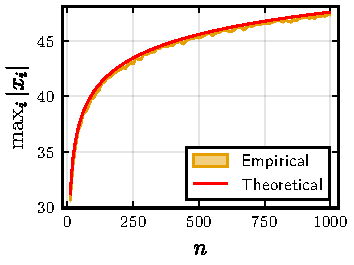
\includegraphics[width=0.9\textwidth]{figures/maxabs_gev.pdf}
        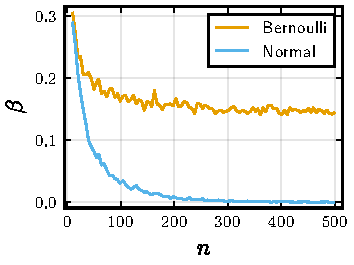
\includegraphics[width=0.9\textwidth]{figures/maxabs_n.pdf}
        \caption{%
          Effects of maximum absolute value scaling.
        }
      \end{figure}
    \end{column}
  \end{columns}

\end{frame}

\end{document}

